% Orchestration decision — "who holds the plan" stop-at-first-match tree.
% Pedagogy pass: terse labels, no command subtitles (prose carries them), color =
% the four surfaces (subagents=blue, agent view=green, agent teams=gold,
% workflows=plum); neutral decision diamonds. Warm-Tol brand hues.
\documentclass[tikz,border=4mm]{standalone}
\usepackage{tikz}
\usetikzlibrary{positioning, shapes.geometric, arrows.meta, calc}

\definecolor{warmblue}{HTML}{3B6FA0}
\definecolor{warmgreen}{HTML}{4A7E3F}
\definecolor{warmgold}{HTML}{C09840}
\definecolor{warmplum}{HTML}{8A4E82}

\begin{document}
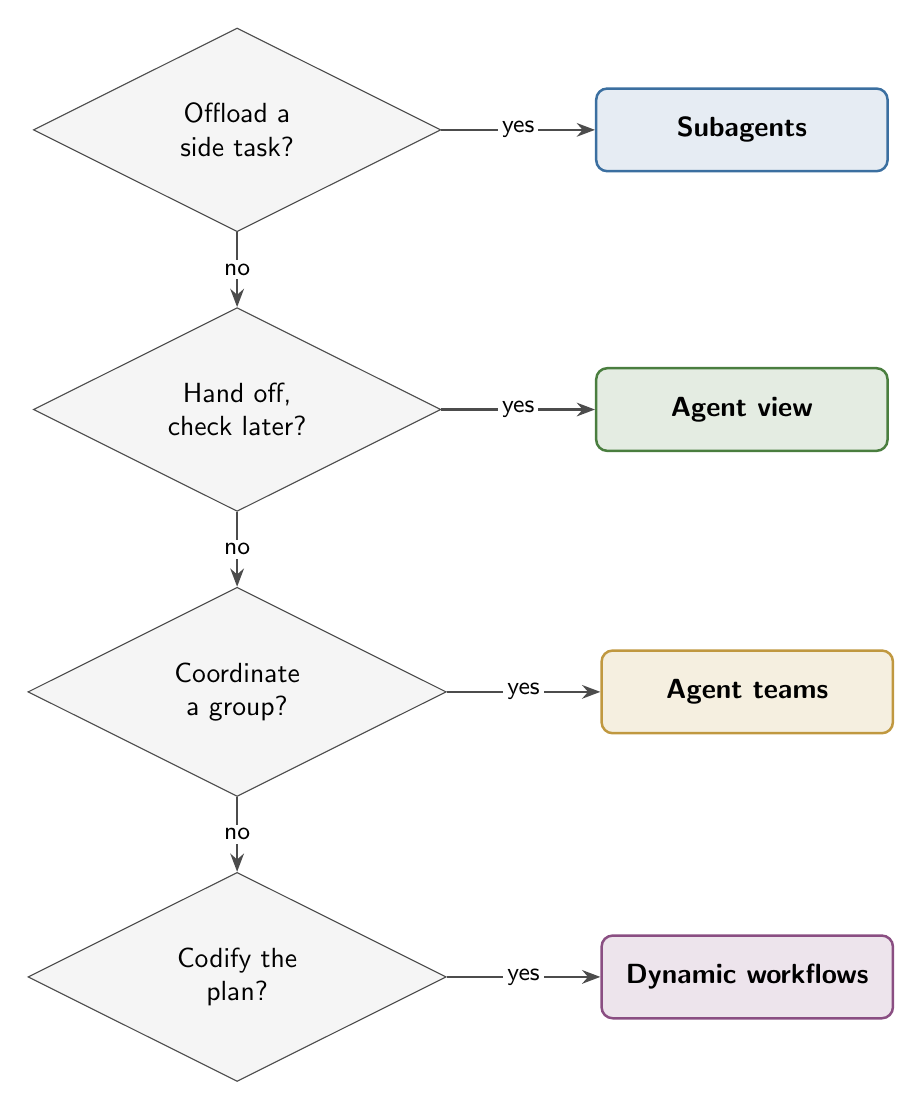
\begin{tikzpicture}[
  font=\sffamily,
  node distance=0.95cm and 1.95cm,
  question/.style={
    draw=gray!60!black, fill=gray!8, diamond, aspect=2.0,
    inner sep=4pt, align=center, text width=3.0cm, font=\sffamily
  },
  ep/.style={
    rounded corners=4pt, minimum width=3.7cm, minimum height=1.05cm,
    inner sep=6pt, align=center, font=\sffamily\bfseries, line width=0.9pt
  },
  epblue/.style={ep, draw=warmblue, fill=warmblue!13},
  epgreen/.style={ep, draw=warmgreen, fill=warmgreen!15},
  epgold/.style={ep, draw=warmgold, fill=warmgold!16},
  epplum/.style={ep, draw=warmplum, fill=warmplum!15},
  arrow/.style={-Stealth, thick, draw=gray!60!black},
  arrowlabel/.style={font=\sffamily\small, fill=white, inner sep=1.5pt},
]

\node[question] (q1) {Offload a \\ side task?};
\node[epblue, right=of q1] (sub) {Subagents};

\node[question, below=of q1] (q2) {Hand off, \\ check later?};
\node[epgreen, right=of q2] (av) {Agent view};

\node[question, below=of q2] (q3) {Coordinate \\ a group?};
\node[epgold, right=of q3] (at) {Agent teams};

\node[question, below=of q3] (q4) {Codify the \\ plan?};
\node[epplum, right=of q4] (wf) {Dynamic workflows};

\draw[arrow] (q1) -- node[arrowlabel] {yes} (sub);
\draw[arrow] (q1) -- node[arrowlabel] {no} (q2);
\draw[arrow] (q2) -- node[arrowlabel] {yes} (av);
\draw[arrow] (q2) -- node[arrowlabel] {no} (q3);
\draw[arrow] (q3) -- node[arrowlabel] {yes} (at);
\draw[arrow] (q3) -- node[arrowlabel] {no} (q4);
\draw[arrow] (q4) -- node[arrowlabel] {yes} (wf);

\end{tikzpicture}
\end{document}
